\documentclass[letterpaper, 12pt]{article}
\usepackage{graphicx} % Required for inserting images
\usepackage{textcomp}
\usepackage{fullpage}
\usepackage{amsmath}
\usepackage{xcolor}
\usepackage{float}
\usepackage{geometry}
\usepackage{biblatex}
\geometry{margin=1in}
\usepackage{enumitem}
\usepackage{microtype}
\usepackage{gensymb}
\usepackage{parskip}
\usepackage{tikz}
\usepackage{caption}
\usepackage{cancel}
\usepackage{nicefrac}


\usepackage{hyperref}
\hypersetup{
  colorlinks=true,        % Enable colored links
  linkcolor=teal,         % Set color for internal links
  citecolor=teal,         % Set color for citations
  filecolor=teal,         % Set color for file links
  urlcolor=teal           % Set color for URLs
}

\usepackage[version=4]{mhchem}

\title{Fischer and Haworth projections}
\date{28 Jun 2025}

\begin{document}

\maketitle

\subsection*{Fischer to Haworth projections}
(linear $\to$ ring)

\begin{enumerate}
\item Number the carbons from the carboxyl end of the molecule. Flip the molecule 90$\degree$ to the right and draw the carbon backbone in a horizontal line. Keep track of the anomeric carbon (usually C1).
\item Draw the open ring structure of the molecule, placing the anomeric carbon at the right end of the ring. The groups at the top (originally left) of the rotated structure will point up, and the groups at the bottom (originally right) of the rotated structure will point down. Remember - ``drop it right down, the rest are left up''
\item The hydroxyl (OH) group on the last chiral carbon will launch a nucleophilic attack on the carbonyl carbon to form the ring. Draw the bond between C1 and C5, and place the hydroxyl group on C1. Draw the O-C bond and place the hydroxyl group on the anomeric carbon.
\end{enumerate}

\subsection*{F to H mechanism}
\begin{itemize}
\item On the open ring, the O attacks the carbon group and closes the ring, leaving the \ce{H+} ion.
\item The \ce{H+} ion subsequently attacks the negatively charged oxygen on the carbonyl carbon, forming a hydroxyl (OH) group.
\item The hydroxyl group on the anomeric carbon (C1) is now in the axial position, while the hydroxyl group on the last chiral carbon (C5) is in the equatorial position.
\item The hydroxyl group on the anomeric carbon can be in either the axial or equatorial position, leading to two possible anomers: alpha ($\alpha$) and beta ($\beta$).
\end{itemize}

\begin{figure}[H]
\centering
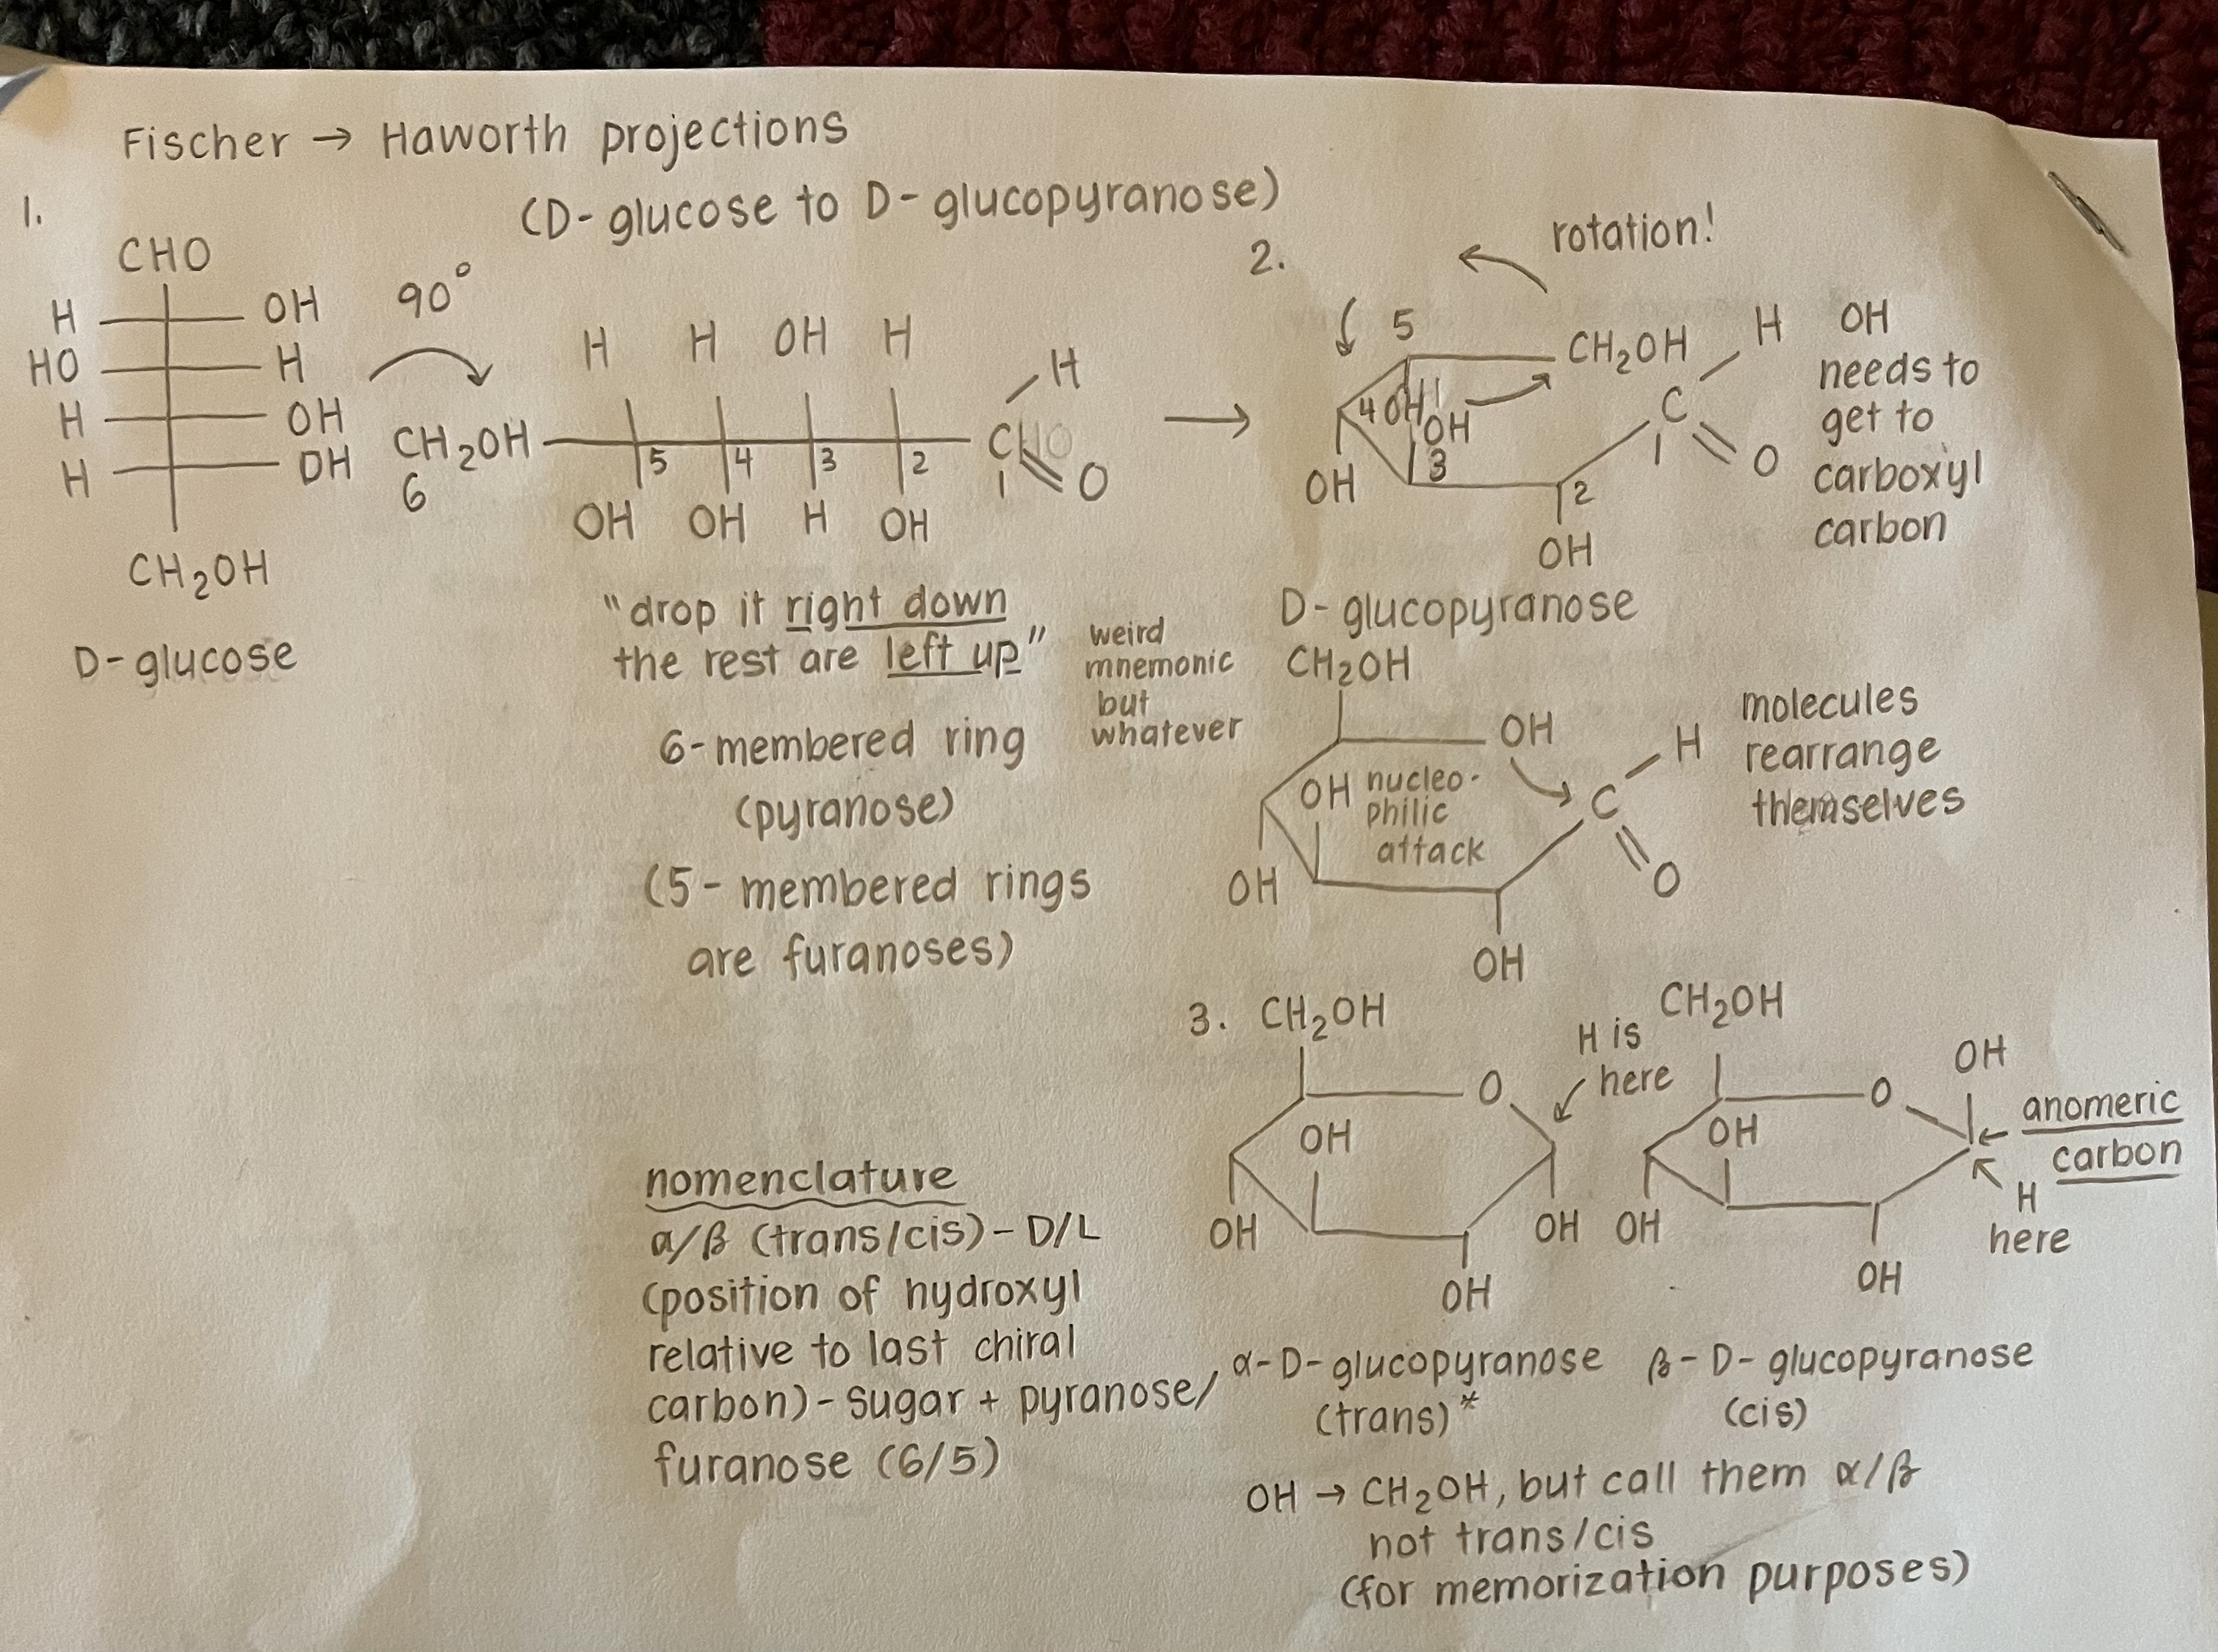
\includegraphics[width=\textwidth]{fth}
\end{figure}

\subsection*{Haworth to Fischer projections}

\begin{enumerate}
\item 
\end{enumerate}

\end{document}